\section{Experimental Results}
\label{sec:Experiments}
\subsection{Variational Auto Encoders}

A very interesting and powerful example of VI is the so-called Variational Auto Encoder (VAE) as introduced by \parencite{Kingma2014} and \parencite{Rezende2014} independently. VAEs are used to estimate the probability density of a set of observations $\{x_i\}_{i=1, \dots, N}$ by assuming the existence of a more concise latent representation or \textit{encoding} $z_i$ for each observed point in some latent space. This model can be trained by optimizing the lower bound $\mathcal{L}$ on the marginal likelihood $p(x_i)$ not only w.r.t.\ the parameters of the posterior approximation, but also w.r.t.\ the parameters of a generative model for $p(x_i, z_i)$ at the same time. Here the generative model usually consists of a fixed prior for the latent variables $\pi(z_i)$ and a conditional distribution or \textit{decoder} $p(x_i|z_i)$ to be learnt. Correspondingly the posterior approximation $q(z_i|x_i)$ is referred to as the \textit{encoder}.

We will in the following apply HMCVI to this model by enhancing the encoder through the addition of some HMC steps and maximizing the auxiliary lower bound $\mathcal{L_\textrm{aux}}$. This should lead to an encoding closer to the best possible encoding given by the true but intractable posterior $p(z_i|x_i)$. Since the HMC steps require the discrete simulation of particle motion on the potential energy surface induced by the generative model, it is recommended to choose $p(x|z)$ to be smooth in order to avoid numerical instabilities and unexpected behaviour.

\subsection{The dataset and the effects of data binarization}
\label{sec:Dataset}
A common benchmark dataset for machine learning problems is the MNIST dataset compiled by \parencite{LeCun1998}, which consists of a total of 70000 $28 \times 28$ pixel images of handwritten digits. The usual modelling approach for probability density estimation of these images is to assume that the pixels follow Bernoulli distributions, so that sampled images are bilevel, i.e.\ only contain the values 0 (black) and 1 (white). However, while the underlying images were bilevel, the images in the dataset contain grey-scales due to the anti-aliasing techniques applied during the normalization preprocessing. To deal with this gap between the bilevel modelling approach and the smoother multilevel dataset several strategies are in use:

The most obvious approach is to simply use the unbinarized original data set (fig.~\ref{fig:MNISTBinarizationComparison}, left), where pixel values range from $0$ to $255/256$ (in $255$ discrete steps). A drawback of this method is its incompatibility with the assumption of a Bernoulli distribution, which leads to a lower likelihood of the model.
% presumably done by \parencite{Kingma2014}
To avoid this incompatibility it is necessary to binarize the images in the dataset. One way to do this is by applying a threshold to the pixel values, so setting the pixel to $1$, if the value is greater or equal to $0.5$, and to $0$ otherwise. This results in very clear images (fig.~\ref{fig:MNISTBinarizationComparison}, middle) and correspondingly a extremely high likelihood for most models. Although this is a very intuitive binarization strategy, it is rarely used in practice.

The most common binarization strategy for MNIST is stochastic binarization, which was introduced by \parencite{Salakhutdinov2008} and has become a standard benchmark for density estimation algorithms \parencite{Salimans2014,Rezende2014}. Here each pixel is randomly set to $1$ with the probability given by its value and to $0$ otherwise, so that taking the average over many draws from the same image returns the original unbinarized image. This procedure can produce somewhat unrealistic digits, which for example have a gaps in the middle of a digit, but still the digits are clearly recognizable (fig.~\ref{fig:MNISTBinarizationComparison}, right). A beneficial side-effect of this randomization is that it counteracts over-fitting to the training set, since the training images appear in many different forms, effectively creating a much larger dataset. In this sense the stochastic binarization acts like dropout regularization \parencite{Hinton2012} built into the dataset. To capitalize on these benefits it is essential to redraw from the training data at the beginning of every epoch. Similarly multiple draws from the validation and test sets should be used for model selection and evaluation in order to obtain robust results. 

\begin{figure}
\centering
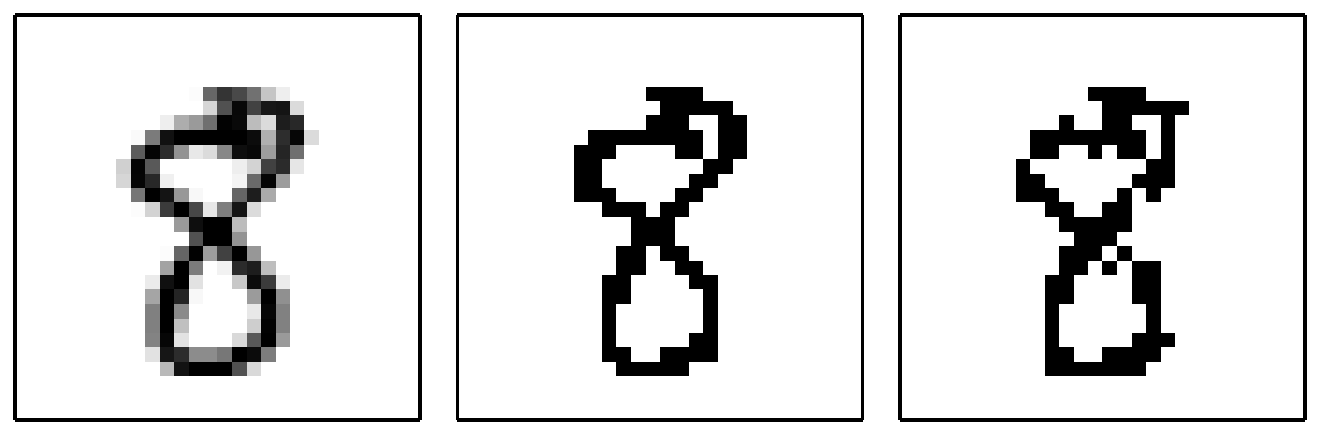
\includegraphics[width=\columnwidth]{figures/binarization_example.pdf}
\caption{Comparison of different binarization strategies on MNIST: The original (left) containing grey-scales was binarized using thresholding (middle) and stochastic binarization (right).}
\label{fig:MNISTBinarizationComparison}
\end{figure}

\subsection{Model Specifications}
\label{sec:ModelSpecifications}
To evaluate HMCVI we will use the MNIST dataset with stochastic binarization for better comparability. The training data was resampled as described above before each iteration. For the validation and test set five random draws from unbinarized sets were used. The HMCVI algorithm was implemented was implemented in python using the package Theano \parencite{Bergstra2010, Bastien2012}. All models were trained for several thousand epochs using Adam \parencite{Kingma2015} integrated with Theano by the package climin \parencite{Bayer2015}. Adam was run with the default parameters except for the step size, which was set to $10^{-4}$ or $5 \cdot 10^{-5}$.

In all experiments the decoding model $p(x_i|z_i)$ consisted of a conditionally independent Bernoulli distribution over the pixels with the rates given by the output of a fully connected neural network with the latent variables as input. This network had two hidden layers with 200 neurons each and softplus ($\log(1 + \exp(x))$) activations. In the output layer the element-wise sigmoid activation function was applied. Similarly for the initial encoder model $q_0(z_i|x_i)$ multivariate normal distribution with diagonal covariance was used, where the parameters are given by the outputs of a second neural network taking the observed variables as inputs. Again two hidden layers with 200 units each were used, here with rectified linear unit (ReLU, $\max(0, x)$) activations. In the output layer the parameters corresponding to the mean were left unchanged, while the variance parameters were passed through the exponential function. As prior distribution for the latent variables a centred isotropic Gaussian distribution was chosen. 

For all HMCVI experiments the leapfrog method was used and the step size learnt (constrained to be positive). In experiments without partial momentum update ($\alpha = 0$ fixed) the reverse momentum model $r_V$ and final momentum model $r_\textrm{final}$ were joined into a single model as explained in section \ref{sec:SimplificationWithoutPartialMomentumUpdate}. This model is like the initial encoder model, but with the previous position and the time step as additional inputs. If partial momentum updates were included, the final momentum model was as in the previous case, but the reverse momentum model $r_V$ was a separate network with the updated momentum as an additional input and otherwise the same specifications as before (see section \ref{sec:TransitionDensitiesNoAcceptance}).

Where an acceptance step was included, either the converged chain approximation ("simple") derived in section \ref{sec:TransDensitiesWithAcceptReverse} was used for the reverse acceptance probability $\mathbb{P}(A = 1|S_t = s_t, t, x)$ or a neural network was trained ("NN"). The output of this neural network, whose final layer was passed through the $\tanh$ function, was added to the converged chain approximation and then clipped to be in $[0, 1]$. The network took the current state, the time step and the observed variables as inputs and consisted of two hidden layers with 200 units each and ReLU activations.

For the canonical momentum distribution, which also specifies the kinetic energy, a zero mean multivariate normal distribution with diagonal covariance matrix was assumed throughout. For the diagonal entries three choices were compared: They were either set to 1 ("Identity") or learnt globally ("Global") or specified by a neural network ("NN") taking the observed variables as input. In the second case the exponential function was applied to unconstrained parameters to ensure positivity. The neural network in the third case had a single hidden layer with 200 units and a ReLU activation and the exponential function as output transfer.

All parameters were independently initialized from a Gaussian distribution $N(0, 0.01)$. In HMCVI experiments the generative model and initial encoder model were then copied from a previously trained VAE (the same for all HMCVI experiments with the same number of latent variables) before training started. With this strategy the HMCVI methods showed much better training results than with fully random initialization.

\subsection{Model Comparison}

\begin{table*}[ht]
\centering
% \begin{tabular}{@{}l@{}c@{}r@{$\;\;\;$}r@{}c@{}r@{$\;\;$}r@{}c@{}r@{}}
% \toprule
% & \phantom{abc}  & \multicolumn{2}{c}{CPU} & \phantom{abc} & \multicolumn{2}{c}{GPU} & \phantom{abc}  & \tn 
% \cmidrule{3-4} \cmidrule{6-7} 
% $r_{z}$ && $e_{rel}$  & $t$ && $e_{rel}$  & $t$ && $M$\tn 
% &&  [$10^{-5}$]  & [ms] && [$10^{-5}$]  & [ms]&& [MB]\tn 

\begin{tabular}{lrrrrrrrr}
\toprule
Name & $d$ & \#HMC & \#LF & Partial & $M$ & Accept & $-\log(p(x)) \leq$ & $- \log(p(x)) \approx$ \tn 
\midrule
Basic VI 2D & 2 & 0 & 0 & - & - & - & 131.76 & 128.95 \tn 
HMCVI 1 & 2 & 1 & 4 & - & Global & - & 130.12 & 127.50 \tn 
HMCVI 2 & 2 & 1 & 12 & - & Global & - & 130.11 & 127.54 \tn 
HMCVI 3 & 2 & 2 & 6 & - & Global & - & 129.78 & 127.27 \tn 
HMCVI 4 & 2 & 3 & 4 & - & Global & - & 129.62 & 127.14 \tn 
HMCVI 5 & 2 & 3 & 4 & Yes & Global & - & 129.25 & 127.03 \tn 
HMCVI 6 & 2 & 3 & 4 & - & Identity & - & 129.59 & 127.11 \tn 
HMCVI 7 & 2 & 3 & 4 & - & NN & - & 129.32 & 127.06 \tn 
HMCVI 8 & 2 & 3 & 4 & Yes & NN & - & 128.96 & 126.94 \tn 
HMCVI 9 & 2 & 3 & 4 & - & Global & Simple & 129.93 & 127.24 \tn 
HMCVI 10 & 2 & 3 & 4 & - & Global & NN & 129.88 & 127.17 \tn 
\midrule
Basic VI 20D & 20 & 0 & 0 & - & - & - & 92.35 & 88.27 \tn 
HMCVI 11 & 20 & 1 & 12 & - & Global & - & 89.77 & 87.77 \tn 
HMCVI 12 & 20 & 2 & 6 & - & Global & - & 89.83 & 87.53 \tn 
HMCVI 13 & 20 & 3 & 4 & - & Global & - & 90.24 & 87.56 \tn 
HMCVI 14 & 20 & 3 & 4 & Yes & Global & - & 90.15 & 87.49 \tn 
HMCVI 15 & 20 & 3 & 4 & - & Identity & - & 91.08 & 87.65 \tn 
HMCVI 16 & 20 & 3 & 4 & - & NN & - & 90.23 & 87.30 \tn 
HMCVI 17 & 20 & 3 & 4 & Yes & NN & - & 89.72 & 87.44 \tn 
HMCVI 18 & 20 & 3 & 4 & - & Global & Simple & 91.40 & 87.28 \tn 
HMCVI 19 & 20 & 3 & 4 & - & Global & NN & 91.37 & 87.32 \tn 
HMCVI 20 & 20 & 3 & 4 & - & NN & Simple & 91.38 & 87.20 \tn 
\bottomrule
\end{tabular}

\caption{Comparison of the obtained lower bound and marginal log-likelihood estimates for different HMCVI configurations with a 2-dimensional (top) and a 20-dimensional latent space (bottom): \#HMC and \#LF give the number of used HMC and leapfrog steps respectively. The "Partial" column indicates, whether partial momentum updates were permitted. The fifth column gives the strategy used for the covariance matrix $M$ of the canonical momentum distribution (as described in section \ref{sec:ModelSpecifications}) and the sixth column, whether the acceptance step was included and if so what approach was used. The last two columns report the lower bound $\mathcal{L_\textrm{aux}}$ and the estimated log-likelihood on the test set.}
\label{tab:Results}
\end{table*}

We maximized the lower bound for various different setups of the HMCVI framework. Table~\ref{tab:Results} shows the results for a two-dimensional latent space and for a 20-dimensional latent space. The negative log-likelihoods given were estimated using importance sampling with 5000 samples (described in appendix~\ref{app:NLLestimateImportSampling}).

From comparing the VAE results to the HMCVI results it is obvious, that any additional HMC steps greatly improve the estimation quality. 

For the two-dimensional latent space we see that increasing the length of the simulated trajectory improves the results and that resampling the momentum more frequently (i.e.\ performing more HMC steps) is also beneficial (compare HMCVI 1 and HMCVI 2-4). From the nature of HMC both of these observations are to be expected, since longer trajectories allow further movement through the latent space and hence better exploration. Likewise more HMC steps means a longer Markov chain, which should thus be closer to convergence. A more intuitive explanation of the second observation is, that initially the simulated particles may have high potential energies and move down the potential energy landscape increasing their kinetic energy. If their large built-up kinetic energy is then reduced by the resampling of the momentum, they can not move out of the potential energy basin they have slid into. Conversely if their is a less frequent resampling of the momentum, their built-up momentum may carry them out of the basin again on the other side, so that their potential energy has not decreased as much and correspondingly their joint likelihood $p(x, z)$ has not increased as much (compare figures~\ref{fig:HMC_Motion_1hmc_12lf} and \ref{fig:HMC_Motion_3hmc_04lf}).

Allowing partial momentum updates and the covariance matrix to depend on the observed variables further improved the performance as expected (HMCVI 5 and 7), with their combination resulting in the best performance (HMCVI 8). Interestingly fixing the covariance matrix to be the identity  (HMCVI 6) performed no worse than learning it globally (HMCVI 4).

Disappointingly, including the acceptance step returned worse results than without it, but as to be expected the more complicated reverse probability model (HMCVI 10) outperformed the approach, where the chain was assumed to have already converged (HMCVI 9). The weaker performance of HMCVI with acceptance step is probably due to the fact, that the short chains being used here have not nearly converged to their invariant distribution. Therefore the reduced mixing due to the rejection of proposals outweighs possible gains from the improved posterior approximation, since only with the acceptance step the chain will actually converge to the true posterior. Additionally the inclusion of the acceptance step significantly raises the computational costs.
